\section{Approach}
\label{sec:Approach}
% We name our technique for CPDP on datasets having
% different metric sets as ``cross-domain defect prediction.'' In this study, we
% define {\em a domain} as the development environment of a software project. The
% reason for different metric sets is due to different development environment.
% For example, we cannot extract the object-oriented metrics from the software
% projects that are not developed in the object-oriented languages. In addition,
% metric values may have different distributions in different development
% environments.
% %  In the machine
% % learning literature, ``different domains'' indicate different feature spaces
% In other words, defect prediction datasets collected from different
% projects developed by various development environments can have different metric sets
% and distributions (i.e. different domains)~\cite{promise12}.
% Thus, our proposed approaches focus on resolving
% the differences between projects from the various domains to improve prediction
% performance.

\begin{figure}[t]
	\centering
	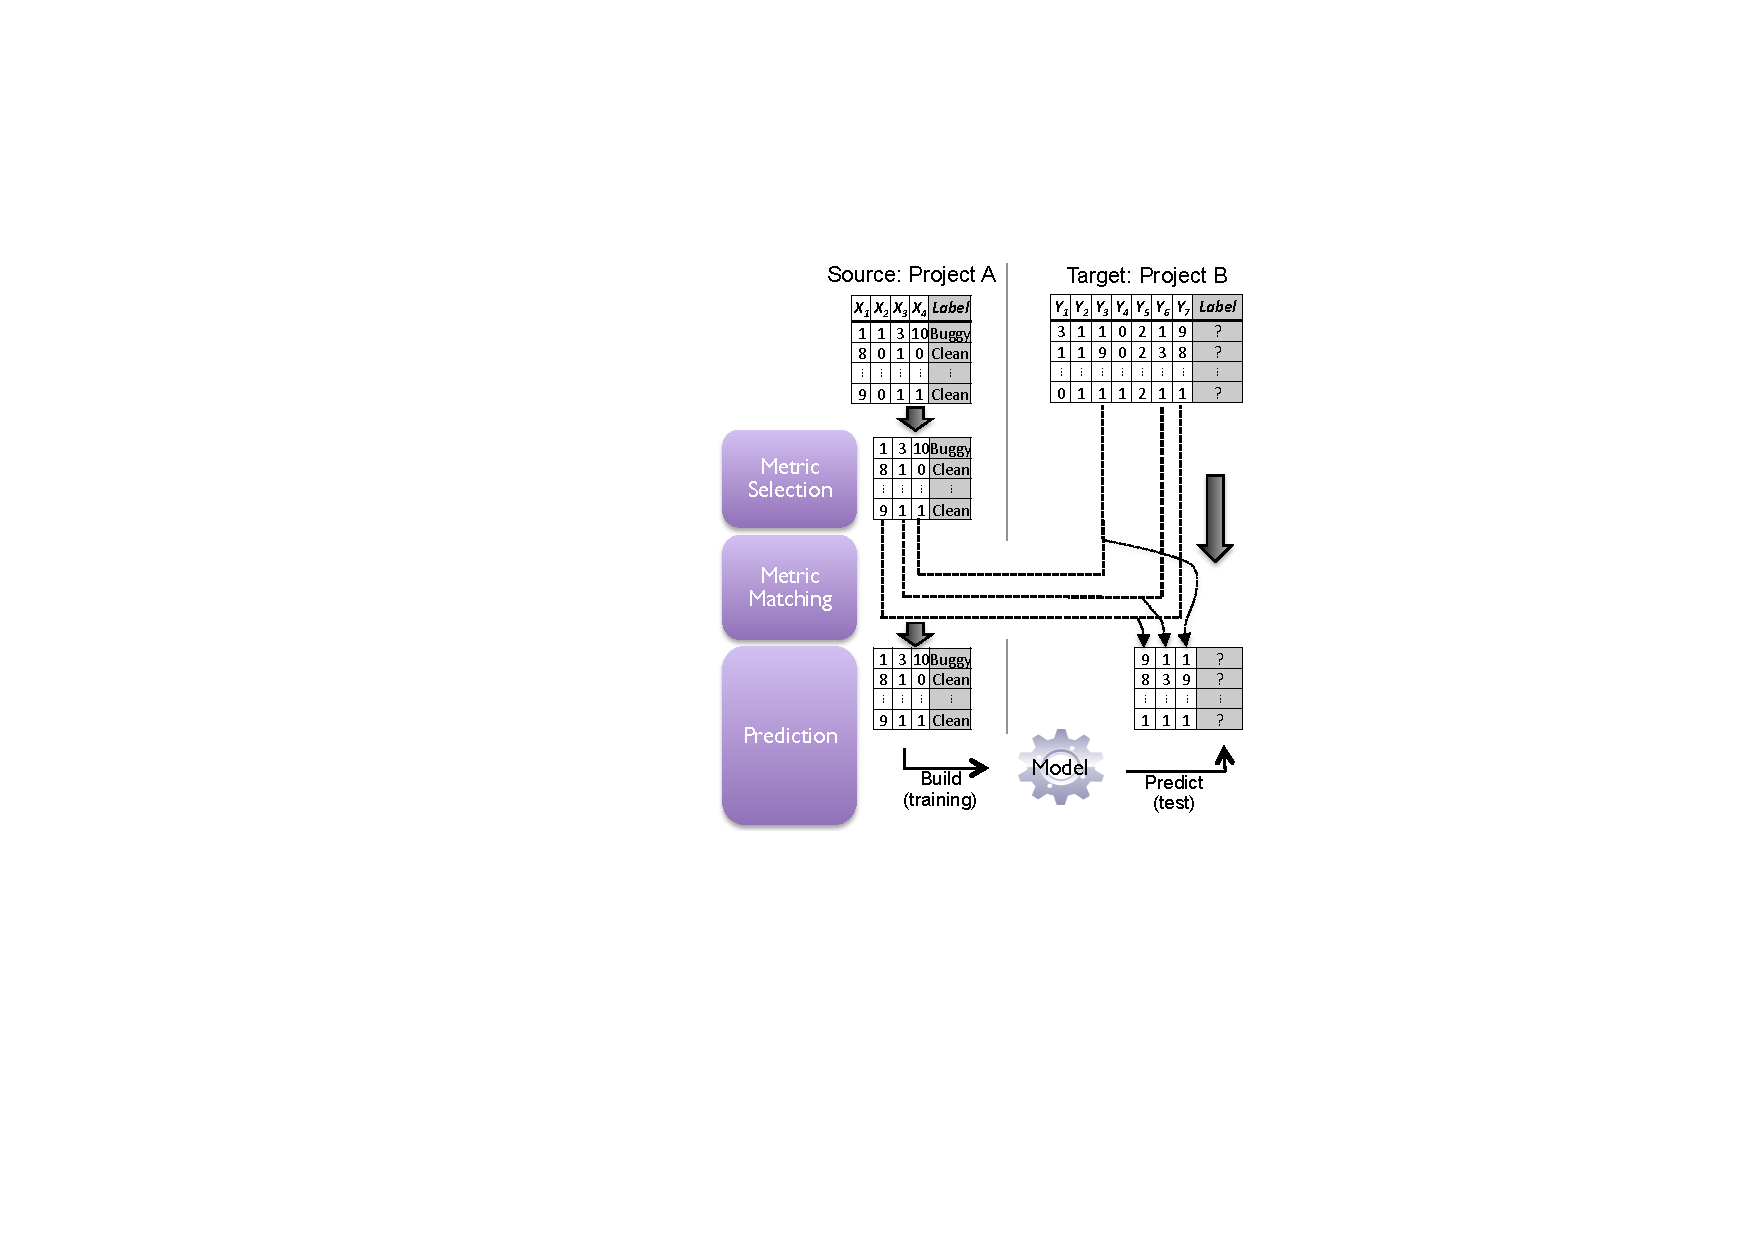
\includegraphics[width=0.925\linewidth]{Figures/framework.pdf}
	\caption{Heterogeneous defect prediction}
	\label{fig:framework}
\end{figure}

Figure~\ref{fig:framework} shows the overview of HDP based on metric selection
and metric matching. In the figure, we have two datasets, Source and Target,
with heterogeneous metric sets. Each row and column of a dataset represents an
instance and a metric, respectively, and the last column represents instance
labels. As shown in the figure, the metric sets in the source and target datasets are not identical ($X_1$ to $X_4$ and $Y_1$ to
$Y_7$ respectively).

When given source and target datasets with heterogeneous metric sets, for metric
selection we first apply a feature selection technique to the source. Feature
selection is a common approach used in machine learning for selecting a subset
of features by removing redundant and irrelevant features~\cite{Guyon03}.
% Since
% software metrics can be considered as features in the machine learning sense,
%by using feature selection techniques.
% As discussed in Section~\ref{sec:Background}, using only common metrics between
% source and target defect datasets to build a prediction model limits the
% prediction performance since informative metrics may not be included in the
% common metric set. To address this issue,
We apply widely used feature selection
techniques for metric selection of a source dataset as in
Section~\ref{sec:metricselection}~\cite{Gao11,Shivaji13}.
% In addition, applying
%feature selection can be helpful to build a better defect prediction
%model~\cite{Shivaji13,Catal09,CHALLAGULLA08}.

After that, metrics based on their similarity such as distribution
or correlation between the source and target metrics are matched up. In
Figure~\ref{fig:framework}, three target metrics are matched with the
same number of source metrics.

After these processes, we finally
arrive at a matched source and target metric set. With the final
source dataset, HDP builds a model and predicts labels of
target instances.

In the following subsections, we explain the metric selection and matching in
detail.

%   \item {\bf Filtering out source features whose median value of buggy
%   instances are lower than that of clean instances}: The intuition of this
%   strategy is based on the unique characteristic of defect prediction datasets,
%   i.e. defect prediction metrics are positively correlated. In other
%   words, typical defect prediction metrics (features) measure the complexity of
%   the source code and development process so that there is a tendency that
%   {\em a higher complexity causes more
%   bug-proneness}~\cite{DAmbros12,Menzies08,Rahman13}. For example, if a
%   source code file has more {\em LOC}, one of complexity measures, then the file may have a higher chance
%   of being bug-prone. This is a typical rationale for defect prediction metrics.
%   However, some features in datasets may not follow this rationale; the lower
%   feature (metric) value, the higher bug-proneness. We regard them as noisy
%   features.~\sung{I don't agree with this. As long as they are correlated it
% is fine. For example, \# of comments. Say more comments leads to less bugs.
% But it's OK. Perhaps, what you did here is another feature selection? You remove non positively correlated features? What would be the results without this process?} Thus, to filter out noisy features, we remove source features whose   median value is lower than that of clean instances. In   Section~\ref{sec:filter}, we describe how to filter out these noisy features
%   in detail.
% \squishend


% Figure~\ref{fig:framework} gives the cross-domain defect
% prediction overview.
% The cross-domain defect prediction consists of four components: label adjuster,
% feature selector, co-occurrence analyzer, and cross-prediction runner.
%
% The label adjuster makes label names between source and target datasets the same
% if they are different. For example, NASA and SOFTLAB defect datasets in the PROMISE
% repository have different buggy (clean) labels, that is, ``Y'' (``N'') and
% ``true'' (``false''), respectively~\cite{promise12}. We convert these different
% label values; ``Y'' and ``true'' as ``buggy'' and ``N'' and ``false'' as ``clean''.

\subsection{Metric Selection in Source Datasets}\label{sect:fss}
\label{sec:metricselection}
For metric selection, we used various feature selection
approaches widely used in defect prediction such as gain ratio, chi-square,
relief-F, and significance attribute evaluation~\cite{Gao11,Shivaji13}. In our experiments, we used Weka implementation for these four feature selection approaches~\cite{Weka}
According to benchmark studies about various feature selection approaches, a
single best feature selection approach for all prediction models does not
exist~\cite{Catal09,Hall03,Liu02}. For this reason, we conduct experiments
under different feature selection approaches. When applying feature selection
approaches, we select top 15\% of metrics as suggested by Gao et
al.~\cite{Gao11}. For example, if the number of features in a dataset is 200, we select 30 top features ranked by a feature selection approach. In addition, we compare the prediction results with or without
metric selection in the experiments.

% The key idea of CFS
%is to select features that highly correlate with class labels but not correlate
% with other features within the same dataset~\cite{Hall98}.  However, we chose CFS since it is fast and widely used in benchmark
%studies~\cite{Menzies07,Catal09,Hall03,Liu02,CHALLAGULLA08}.
%  Hall
% proposed the CfsSubsetEval algorithm by combining a correlation measure and a heuristic
% search technique~\cite{Hall98}.



% It is possible to use other feature selection
% approaches~\cite{Shivaji13}. However, we used the CfsSubsetEval in our
% experimental setting for easy replication since
% the CfsSubsetEval is a Weka's default feature selection
% algorithm~\cite{Weka}.~\sung{This is very weak argument. As long as other algorithms are available, they can replicate. Provide other reasons. Perhaps, this algorithm is simple?fast? many others are using this?}

\subsection{Matching Source and Target Metrics}
%  based on
% distribution similarity}
\label{sec:analyzers}

Matching source and target metrics is the core of HDP.
The intuition of matching metrics is originated from the typical defect-proneness tendency of software metrics, i.e., the higher complexity of source code and development process causes the more defect-proneness~\cite{Menzies07,DAmbros12,nam2015clami}. The higher complexity of source code and development process is usually represented with the higher metric values. Thus, various product and process metrics, e.g., McCabe's cyclomatic, lines of code, and the number of developers modifying a file, follow this defect-proneness tendency~\cite{Bird2011,DAmbros12,Menzies07,Ohlsson1996,Rahman13}. By matching metrics, HDP transfers this defect-proneness tendency from a source project for predicting defects in a target project. For example, assume that a metric, the number of methods invoked by a class ({\em RFC}), in a certain Java project (source) has the tendency that a class file having the RFC value greater than 40 is highly defect-prone. If a target metric, {\em the number of operands}, follows the similar distribution and its defect-proneness tendency, transferring this defect-proneness tendency of the source metric, RFC, as knowledge by matching the source and target metrics could be effective to predict defects in the target dataset.

To match source and target metrics, we measure the similarity of each source and
target metric pair by using several existing methods such as percentiles,
Kolmogorov-Smirnov Test, and Spearman's correlation
coefficient~\cite{Massey51,Spearman10}.
We define metric matching analyzers as follows:
\squishlist
	\item Percentile based matching (PAnalyzer)
	\item Kolmogorov-Smirnov Test based matching (KSAnalyzer)
	\item Spearman's correlation based matching (SCoAnalyzer)
	%\item Popularity index based matching (PiAnalyzer)
\squishend

% \begin{figure}[t]
% 	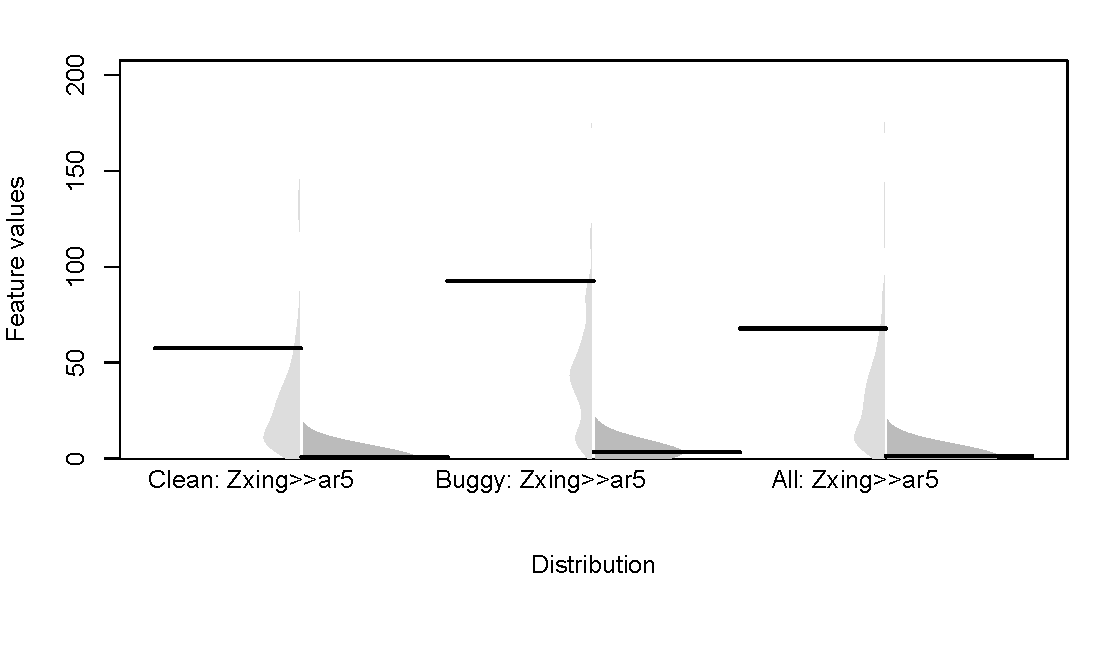
\includegraphics[width=\linewidth]{Figures/Result/beanplot_manual_matching.pdf}
% 	\caption{Feature value distribution of a common feature, `{\em lines of code
% 	and comments}', between datasets, Zxing and ar5. The three plots shows feature
% 	value distributions for clean, buggy, and all instances respectively. A solid
% 	horizontal line represents an average feature value for each plot.}
% 	\label{fig:common_feature}
% \end{figure}
%
% % To build efficient machine learning models, the distribution of both
% %   training and test data should be same~\cite{Pan10}.However,
% %   datasets from different domains most likely have different distributions.
%
% Since researchers in previous studies of cross-project defect prediction focused
% on making different features similar or selecting similar instances, similarity
% between source and target datasets is an important factor for
% cross-prediction~\cite{Nam13,Ma12,Turhan09,Watanabe08}. How
% Figure~\ref{fig:common_feature} shows distributions of a feature, `{\em lines of code and comments}', in two datasets, Zxing and ar5. In the figure, the light grey areas represent the feature value distribution of Zxing and the dark
% grey areas are for ar5. Three sets of plots show feature distributions of clean,
% buggy, and all (both buggy and clean) instances. As in
% Figure~\ref{fig:common_feature}, feature distributions between Zxing and ar5 are
% very different although it is the same metric, `{\em lines of code and
% comments}'. For this reason, we avoid using common features between two datasets.
% Instead, we just match features between
% source and target datasets based on their similarities, and the
% matched features for defect prediction.
% In Section~\ref{sec:analyzers}, we explain four
% feature matching approaches.
% \item

%\subsection{Cross-domain Defect Prediction Model}
%\label{sec:framework}


% In case that a dataset
% has nominal, ordinal, or cardinal values as labels, we should transform the
% values into binary class labels. For example, if a dataset have ten cardinal
% label values from 1 to 10, we can set a cutoff value for a buggy label. Assuming
% the cutoff value for a buggy label is 5, we can label instances with the values
% below 5 or same as 5 as buggy, otherwise as clean.
% Label adjusting is a very preliminary step to build a cross-domain prediction
% model.

\begin{figure}[t]
	\centering
	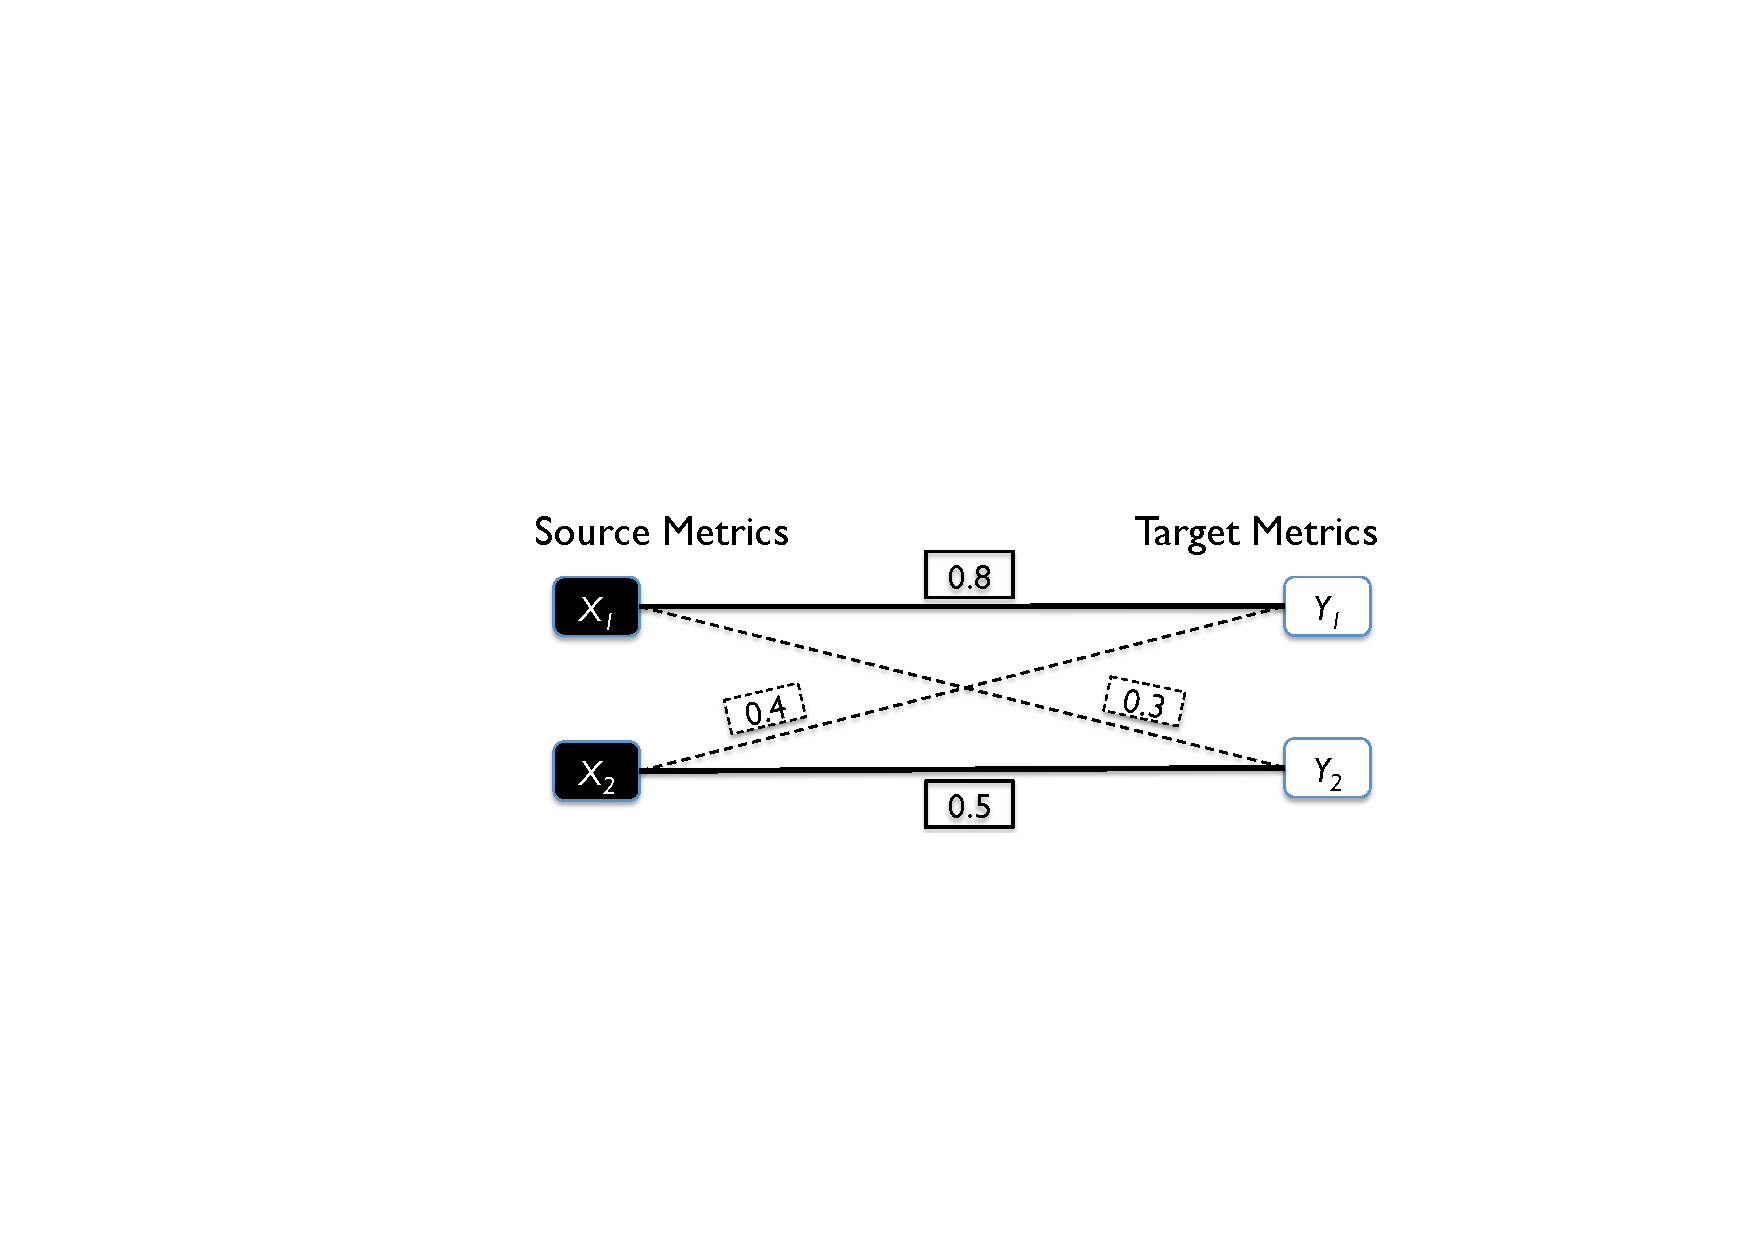
\includegraphics[width=\linewidth]{Figures/matching.pdf}
	\caption{An example of metric matching between source and target
	datasets.}
	\label{fig:matching}
\end{figure}

The key idea of these analyzers is computing matching
scores for all pairs between the source and target metrics.
Figure~\ref{fig:matching} shows a sample
matching. There are two source metrics ($X_1$ and $X_2$) and
two target metrics ($Y_1$ and $Y_2$). Thus, there are four possible matching
pairs, ($X_1$,$Y_1$), ($X_1$,$Y_2$), ($X_2$,$Y_1$), and ($X_2$,$Y_2$). The
numbers in rectangles between matched source and target metrics in
Figure~\ref{fig:matching} represent matching scores computed by an analyzer. For example,
the matching score between the metrics, $X_1$ and $Y_1$, is 0.8.

From all pairs between the source and target metrics, we remove poorly matched
metrics whose matching score is not greater than a specific cutoff threshold.
For example, if the matching score cutoff threshold is 0.3, we include only the
matched metrics whose matching score is greater than 0.3. In
Figure~\ref{fig:matching}, the edge ($X_1$,$Y_2$) in matched metrics will be
excluded when the cutoff threshold is 0.3. Thus, all the candidate matching
pairs we can consider include the edges ($X_1$,$Y_1$), ($X_2$,$Y_2$), and
($X_2$,$Y_1$) in this example.
In Section~\ref{sec:Evaluation}, we design our empirical study under different
matching score cutoff thresholds to investigate their impact on prediction.

We may not have any matched metrics based on the cutoff threshold. In this
case, we cannot conduct defect prediction. In
Figure~\ref{fig:matching}, if the cutoff threshold is 0.9, none of the matched
metrics are considered for HDP so we cannot build a prediction model for the target
dataset. For this reason, we investigate target prediction coverage (i.e.,
what percentage of target datasets could be predicted?) in
our experiments.

After applying the cutoff threshold, we
used {\em the maximum weighted bipartite matching}~\cite{Matouek06} technique to
select a group of matched metrics, whose sum of matching scores is highest,
without duplicated metrics.
%We can form groups of matched features without redundant features.
In Figure~\ref{fig:matching}, after applying the cutoff threshold of 0.30, we
can form two groups of matched metrics without duplicated metrics. The first
group consists of the edges, ($X_1$,$Y_1$) and ($X_2$,$Y_2$), and another group
consists of the edge ($X_2$,$Y_1$). In each group, there are no duplicated
metrics. The sum of matching scores in the first group is 1.3 (=0.8+0.5) and that of the second
group is 0.4.
The first group has a greater sum (1.3) of matching scores than the
second one (0.4). Thus, we select the first matching group as the set of
matched metrics for the given source and target metrics with the cutoff
threshold of 0.30 in this example.
%that can be solved
% by a linear program in polynomial time~\cite{Matouek06}.

% Based on the co-occurrence features, we can
% generate new source and target datasets with only the co-occurrence features.
% For example, as shown in Figure~\ref{fig:framework}, the datasets of Project A
% and B have three (after feature selection) and eight features respectively and
% two sets of features (dashed lines) are identified as co-occurrence features. With
% these co-occurrence features, we can generate new source and target datasets
% with a two-feature set as in Figure~\ref{fig:framework}. We designed various
% co-occurrence analyzers, which are explained in Section~\ref{sec:analyzers}.
%


% as
% explained in Section~\ref{sec:Background}. Among them, we use
% ASAnalyzer with Filters investigated in Section~\ref{sec:ASAnalyzer}.

% The cross-prediction runner conducts actual cross-domain defect prediction. The
% runner builds a prediction model by using a new source dataset and predicts
% the defects on a new target dataset. To our knowledge, cross-domain defect
% prediction is the first study on defect prediction using datasets with different
% feature spaces.


% \subsection{Feature Matching Analyzers} %Identifying co-occurrence features}
% \label{sec:analyzers}
% To identify co-occurrence features between source and target datasets, we
% design five co-occurrence feature analyzers as follows:
% \squishlist
% 	\item Average and Standard deviation analyzer (ASAnalyzer)
% 	\item T-test analyzer (TAnalyzer)
% 	\item Pearson's correlation analyzer
% (PCoAnalyzer)
% 	\item Spearman's correlation analyzer (SCoAnalyzer)
% 	\item Popularity index analyzer (PiAnalyzer)
% \squishend

% Before applying analyzers, all feature values
% of datasets are normalized between 0 and 1 to avoid no individual feature has
% greater influence than others~\cite{Kocaguneli13}.

Each analyzer for the metric matching scores is described in the following subsections.

\subsubsection{PAnalyzer}
PAnalyzer simply compares 9 percentiles (10th, 20th,\ldots, 90th) of ordered
values between source and target metrics. A percentile is a statistical measure that indicates the value at a specific percentage of observations in descriptive statistics. By comparing differences at the 9 percentiles, we simulate the similarity between source and target metric values. The intuition of this analyzer comes from the assumption that the similar source and target metric values have similar statistical information. Since comparing only medians, i.e., 50th percentile just show one aspect of distributions of source and target metric values, we expand the comparison at the 9 spots of distributions of those metric values.

First, we compute the difference of $n$-th
percentiles in source and target metric values by the following
equation:
\begin{equation}
P_{ij}(n)=\frac{sp_{ij}(n)}{bp_{ij}(n)}
\end{equation}
where $P_{ij}(n)$ is the comparison function for $n$-th percentiles
of $i$-th source and $j$-th target metrics, and $sp_{ij}(n)$ and $bp_{ij}(n)$
are smaller and bigger percentile values respectively at $n$-th percentiles
of $i$-th source and $j$-th target metrics. For example, if the 10th
percentile of the source metric values is 20 and that of target metric values is
15, the difference is 0.75 ($P_{ij}(10)=15/20=0.75$). Then, we repeat this calculation at the 20th, 30th,\ldots, 90th percentiles.

Using this percentile comparison function, a matching score between source
and target metrics is calculated by the following equation:
\begin{equation}
M_{ij}=\frac{\sum\limits_{k=1}^9
P_{ij}(10\times{k})}{9}\end{equation}
where $M_{ij}$ is a matching score between $i$-th source and $j$-th
target metrics. For example, if we assume a set of all $P_{ij}$, i.e., $P_{ij}{(10\times{k})}=\{0.75, 0.34, 0.23, 0.44, 0.55, 0.56, 0.78, 0.97, 0.55\}$, $M_{ij}$ will be 0.574(=$\frac{0.75+0.34+0.23+0.44+0.55+0.56+0.78+0.97+0.55}{9}$). The best matching score of this equation is 1.0
when the values of the source and target metrics of all 9 percentiles are the
same, i.e., $P_{ij}(n)=1$.

\subsubsection{KSAnalyzer}

KSAnalyzer uses a p-value from the Kolmogorov-Smirnov Test (KS-test) as a matching score between source and target metrics. The KS-test is a non-parametric statistical test to compare two samples~\cite{Lilliefors67,Massey51}. Particularly, the KS-test can be applicable when we cannot be sure about the normality of two samples and/or the same variance~\cite{Lilliefors67,Massey51}. Since metrics in some defect datasets used in our empirical study have exponential distributions~\cite{Menzies07} and metrics in other datasets have unknown distributions and variances, the KS-test is a suitable statistical test to compare two metrics.

In the KS-test, a p-value shows the significance level with which we have very strong evidence to reject the null hypothesis, i.e., two samples are drawn from the same distribution~\cite{Lilliefors67,Massey51}. We expected that matched metrics whose null hypothesis can be rejected with significance levels specified by commonly used p-values such as 0.01, 0.05, and 0.10 can be filtered out to build a better prediction model. Thus, we used a p-value of the KS-test to decide the matched metrics should be filtered out. We used the {\em KolmogorovSmirnovTest} implemented in the {\em Apache commons math3 3.3} library.

The matching score is:
\begin{equation}M_{ij}=p_{ij}\end{equation}
where $p_{ij}$ is a p-value from the KS-test of $i$-th source and $j$-th
target metrics. Note that in KSAnalyzer the higher matching score does not represent the higher similarity of two metrics. To observe how the matching scores based on the KS-test impact on prediction performance, we conducted experiments with various p-values.

\subsubsection{SCoAnalyzer}
In SCoAnalyzer, we used the Spearman's
rank correlation coefficient as a matching score for source and target
metrics~\cite{Spearman10}.
Spearman's rank correlation measures how two samples
are correlated~\cite{Spearman10}. To compute the coefficient, we used the
{\em SpearmansCorrelation} in the {\em Apache commons math3 3.3} library. Since the
size of metric vectors should be the same to compute the coefficient, we
randomly select metric values from a metric vector that is of a greater size
than another metric vector. For example, if the sizes of the source and target metric
vectors are 110 and 100 respectively, we randomly select 100 metric values from the
source metric to agree to the size between the source and target metrics. All
metric values are sorted before computing the coefficient.

The matching score is as follows:
\begin{equation}M_{ij}=c_{ij}\end{equation}
where $c_{ij}$ is a Spearman's rank correlation coefficient between $i$-th
source and $j$-th target metrics.

% \subsubsection{Popularity Index (PiAnalyzer)}
% We adopted the
% concept of popularity index to identify similar source and target
% metrics~\cite{Kocaguneli13}.
% The popularity index was proposed by Kocaguneli et al. to discard redundant
% metrics and outlier instances for effort estimation~\cite{Kocaguneli13}.
% Popularity index represents how many times a metric or an instance is a nearest
% neighbor of other metrics or instances~\cite{Kocaguneli13}.
%
% To match source and target
% metrics based on the popularity index, we proceed with the following steps:
% \squishlist
%   \item{Step 1:} Select and sort source and target instances by popularity
%   index.\footnote{Please, refer to the study of Kocaguneli et al.
% for details of the popularity index~\cite{Kocaguneli13}.}
%   This selection process makes the number of instances same in both source and
%   target datasets.
%   \item {Step 2:} Compute a matching score for each pair of source and target
%   metrics in the datasets consisting of instances from Step 1. The matching
%   score is:
% 		\begin{equation}M_{ij}=1-norm(E_{ij})\end{equation}
% 	where $E_{ij}$ is a Euclidean distance between $i$-th source and $j$-th
% 	target metrics and $norm(x)$ is the normalization function to make $x$ range
% 	from zero to one. The matching score tends to be one when the distance between $i$-th source and $j$-th
% 	target metrics, $E_{ij}$, is closest.
% 	\item {Step 3:} Find a nearest neighbor of each source metric by using
% 	sorted matching scores from Step 2.
% \squishend
% After executing Step 3, we can match metrics between the
% source and target based on the popularity index.

% \begin{table}[t]
% \small
% \centering
% \caption{Comparison of Co-occurrence analyzers in terms of average AUC for
% 600 cross predictions from 28 defect datasets. (The matching score cutoff is
% 0.00. This means we use all matched features for training and test models.)}
% \label{tab:DiffAnalyzers}
% %\setlength{\tabcolsep}{5pt}
% %\setlength{\extrarowheight}{1.5pt}
% \begin{tabular}{|c|c|}
% \hline
% Analyzer	& Average AUC	\\\hline \hline
% ASAnalyzer	& 0.58	\\\hline
% TAnalyzer	& 0.58	\\\hline
% PCoAnalyzer	& 0.52	\\\hline
% SCoAnalyzer	& 0.51	\\\hline
% PiAnalyzer	& 0.57	\\\hline
% \end{tabular}
% \end{table}

\subsection{Building Prediction Models}

After applying metric selection and matching, we can finally build a
prediction model using a source dataset with selected and matched metrics. Then,
as a regular defect prediction model, we can predict defects on a target dataset
with the matched metrics.
